% ----------------------------------------------------------
% Apêndices (opcionais)
% ----------------------------------------------------------
% ---
% Inicia os apêndices
% ---
\appendix


%=====================================================================
\postextualchapter{Documentos de casos de uso}\label{ap2}
%=====================================================================
Neste apêndice estão todos os documentos de casos de uso gerado pelo Diagrama de casos de uso.

\begin{table}[!ht]{14cm}
  \caption{Caso de uso Ler Projeto.}
    \begin{tabular}{cc}
    \hline
    \rowcolor[HTML]{333333} 
    {\color[HTML]{FFFFFF} \textbf{Nome do caso de uso}} & {\color[HTML]{FFFFFF} \textbf{Ler Projeto}} \\ \hline
    \rowcolor[HTML]{EFEFEF} 
    \begin{tabular}[c]{@{}c@{}}1.Caso de uso geral\end{tabular} & \begin{tabular}[c]{@{}c@{}} \end{tabular} \\
    \begin{tabular}[c]{@{}c@{}}2.Ator principal \end{tabular} & \begin{tabular}[c]{@{}c@{}} Anônimo\end{tabular} \\
    \rowcolor[HTML]{EFEFEF} 
    \begin{tabular}[c]{@{}c@{}}3.Ator secundário\end{tabular} & \begin{tabular}[c]{@{}c@{}} Aluno, Professor e\\ Administrador\end{tabular} \\
    \begin{tabular}[c]{@{}c@{}}4.Resumo\end{tabular} & \begin{tabular}[c]{@{}c@{}}Este caso de uso consiste na leitura,\\ ou visualização, de um projeto armazenado\\no bando de dados.\end{tabular} \\
    \rowcolor[HTML]{EFEFEF} 
    \begin{tabular}[c]{@{}c@{}}5.Pré-condição\end{tabular} & \begin{tabular}[c]{@{}c@{}}Existir dados públicos \\armazenados no banco de dados\end{tabular} \\
    \begin{tabular}[c]{@{}c@{}}6.Ações do ator\\ I-Acessar banco\\III-Informar login e senha\\ \\ \\VI-Fazer consulta\end{tabular} & \begin{tabular}[c]{@{}c@{}} -Ações do sistema-\\II-Pedir usuário e senha\\IV-Verificar usuário e senha\\V-Permitir acesso de acordo com as restrições \\de tipo de usuário\\ VII- Retornar os dados consultados \end{tabular} \\ 
    \rowcolor[HTML]{EFEFEF} 
    \begin{tabular}[c]{@{}c@{}}7.Restrições e validações
    \end{tabular} & \begin{tabular}[c]{@{}c@{}} O projeto em que contém\\ os dados deve ser público \end{tabular} \\ \hline
    \end{tabular}
  \source{A autora, 2019.}
\end{table}

\begin{table}[!ht]{14cm}
  \caption{Caso de uso Criar Projeto.}
    \begin{tabular}{cc}
    \hline
    \rowcolor[HTML]{333333} 
    {\color[HTML]{FFFFFF} \textbf{Nome do caso de uso}} & {\color[HTML]{FFFFFF} \textbf{Criar Projeto}} \\ \hline
    \rowcolor[HTML]{EFEFEF} 
    \begin{tabular}[c]{@{}c@{}}1.Caso de uso geral\end{tabular} & \begin{tabular}[c]{@{}c@{}} \end{tabular} \\
    \begin{tabular}[c]{@{}c@{}}2.Ator principal \end{tabular} & \begin{tabular}[c]{@{}c@{}}Aluno\end{tabular} \\
    \rowcolor[HTML]{EFEFEF} 
    \begin{tabular}[c]{@{}c@{}}3.Ator secundário\end{tabular} & \begin{tabular}[c]{@{}c@{}}Professor e Administrador\end{tabular} \\
    \begin{tabular}[c]{@{}c@{}}4.Resumo\end{tabular} & \begin{tabular}[c]{@{}c@{}}Este caso de uso consiste na criação\\de um projeto novo dentro do banco de dados \end{tabular} \\
    \rowcolor[HTML]{EFEFEF} 
    \begin{tabular}[c]{@{}c@{}}5.Pré-condição\end{tabular} & \begin{tabular}[c]{@{}c@{}}O login do usuáio ter sido criado\end{tabular} \\
    \begin{tabular}[c]{@{}c@{}}6.Ações do ator\\ I-Acessar banco\\III-Informar login e senha\\ \\ \\VI-Pedir criaação do projeto\end{tabular} & \begin{tabular}[c]{@{}c@{}} -Ações do sistema-\\II-Pedir usuário e senha\\IV-Verificar usuário e senha\\V-Permitir acesso de acordo com as restrições \\de tipo de usuário\\ VII- Criar projeto\end{tabular} \\ 
    \rowcolor[HTML]{EFEFEF} 
    \begin{tabular}[c]{@{}c@{}}7.Restrições e validações
    \end{tabular} & \begin{tabular}[c]{@{}c@{}} O login não ser anônimo \end{tabular} \\ \hline
    \end{tabular}
  \source{A autora, 2019.}
\end{table}

\begin{table}[!ht]{14cm}
  \caption{Caso de uso Editar Projeto.}
    \begin{tabular}{cc}
    \hline
    \rowcolor[HTML]{333333} 
    {\color[HTML]{FFFFFF} \textbf{Nome do caso de uso}} & {\color[HTML]{FFFFFF} \textbf{Editar Projeto}} \\ \hline
    \rowcolor[HTML]{EFEFEF} 
    \begin{tabular}[c]{@{}c@{}}1.Caso de uso geral\end{tabular} & \begin{tabular}[c]{@{}c@{}} \end{tabular} \\
    \begin{tabular}[c]{@{}c@{}}2.Ator principal \end{tabular} & \begin{tabular}[c]{@{}c@{}}Aluno\end{tabular} \\
    \rowcolor[HTML]{EFEFEF} 
    \begin{tabular}[c]{@{}c@{}}3.Ator secundário\end{tabular} & \begin{tabular}[c]{@{}c@{}}Professor e Administrador \end{tabular} \\
    \begin{tabular}[c]{@{}c@{}}4.Resumo\end{tabular} & \begin{tabular}[c]{@{}c@{}} Este caso de uso consiste no\\ armazenamento e edição de dados\\em um banco de dados\end{tabular} \\
    \rowcolor[HTML]{EFEFEF} 
    \begin{tabular}[c]{@{}c@{}}5.Pré-condição\end{tabular} & \begin{tabular}[c]{@{}c@{}}Existir um projeto\end{tabular} \\
    \begin{tabular}[c]{@{}c@{}}6.Ações do ator\\ I-Executar comando de \\armazenamento de dados\\III-Executar comano de edição \\de dados\end{tabular} & \begin{tabular}[c]{@{}c@{}} -Ações do sistema-\\II-Gravar dados\\ \\IV-Editar dados\\ \\V-armazenr alterações nos dados\end{tabular} \\ 
    \rowcolor[HTML]{EFEFEF} 
    \begin{tabular}[c]{@{}c@{}}7.Restrições e validações
    \end{tabular} & \begin{tabular}[c]{@{}c@{}}Projeto deve ser\\ de domínio do usuário\end{tabular} \\ \hline
    \end{tabular}
  \source{A autora, 2019.}
\end{table}

\begin{table}[!ht]{14cm}
  \caption{Caso de uso Deletar Projeto.}
    \begin{tabular}{cc}
    \hline
    \rowcolor[HTML]{333333} 
    {\color[HTML]{FFFFFF} \textbf{Nome do caso de uso}} & {\color[HTML]{FFFFFF} \textbf{Deletar Projeto}} \\ \hline
    \rowcolor[HTML]{EFEFEF} 
    \begin{tabular}[c]{@{}c@{}}1.Caso de uso geral\end{tabular} & \begin{tabular}[c]{@{}c@{}} \end{tabular} \\
    \begin{tabular}[c]{@{}c@{}}2.Ator principal \end{tabular} & \begin{tabular}[c]{@{}c@{}}Aluno\end{tabular} \\
    \rowcolor[HTML]{EFEFEF} 
    \begin{tabular}[c]{@{}c@{}}3.Ator secundário\end{tabular} & \begin{tabular}[c]{@{}c@{}}Professor e Administrador \end{tabular} \\
    \begin{tabular}[c]{@{}c@{}}4.Resumo\end{tabular} & \begin{tabular}[c]{@{}c@{}}Este caso de consiste no ato\\ de deletar um projeto do banco de dados \end{tabular} \\
    \rowcolor[HTML]{EFEFEF} 
    \begin{tabular}[c]{@{}c@{}}5.Pré-condição\end{tabular} & \begin{tabular}[c]{@{}c@{}}Existir um projeto\end{tabular} \\
    \begin{tabular}[c]{@{}c@{}}6.Ações do ator\\ I-Executar comando que delete\\ o projeto\end{tabular} & \begin{tabular}[c]{@{}c@{}} -Ações do sistema-\\II-Deletar projeto\\  \end{tabular} \\ 
    \rowcolor[HTML]{EFEFEF} 
    \begin{tabular}[c]{@{}c@{}}7.Restrições e validações
    \end{tabular} & \begin{tabular}[c]{@{}c@{}}Projeto deve ser de domínio\\do usuário\end{tabular} \\ \hline
    \end{tabular}
  \source{A autora, 2019.}
\end{table}

\begin{table}[!ht]{14cm}
  \caption{Caso de uso Criar Usuário Nível 2.}
    \begin{tabular}{cc}
    \hline
    \rowcolor[HTML]{333333} 
    {\color[HTML]{FFFFFF} \textbf{Nome do caso de uso}} & {\color[HTML]{FFFFFF} \textbf{Criar Usuário Nível 2}} \\ \hline
    \rowcolor[HTML]{EFEFEF} 
    \begin{tabular}[c]{@{}c@{}}1.Caso de uso geral\end{tabular} & \begin{tabular}[c]{@{}c@{}} \end{tabular} \\
    \begin{tabular}[c]{@{}c@{}}2.Ator principal \end{tabular} & \begin{tabular}[c]{@{}c@{}}Professor\end{tabular} \\
    \rowcolor[HTML]{EFEFEF} 
    \begin{tabular}[c]{@{}c@{}}3.Ator secundário\end{tabular} & \begin{tabular}[c]{@{}c@{}}Aluno\end{tabular} \\
    \begin{tabular}[c]{@{}c@{}}4.Resumo\end{tabular} & \begin{tabular}[c]{@{}c@{}}Este caso de uso consiste na\\ criação de um usuário do nível 2\end{tabular} \\
    \rowcolor[HTML]{EFEFEF} 
    \begin{tabular}[c]{@{}c@{}}5.Pré-condição\end{tabular} & \begin{tabular}[c]{@{}c@{}}Login do usuário ser\\ Professor ou Administrador\end{tabular} \\
    \begin{tabular}[c]{@{}c@{}}6.Ações do ator\\ I-Preencher dados de novo usuário\\II-Mandar criar novo usuário\\ \\ \\ \\\end{tabular} & \begin{tabular}[c]{@{}c@{}} -Ações do sistema-\\ \\III-Checar se o usuário tem permissão \\ para criai o usuário nível 2\\IV-Criar usuário\end{tabular} \\ 
    \rowcolor[HTML]{EFEFEF} 
    \begin{tabular}[c]{@{}c@{}}7.Restrições e validações
    \end{tabular} & \begin{tabular}[c]{@{}c@{}}O usuário a ser criado\\ deve se de nível 2\end{tabular} \\ \hline
    \end{tabular}
  \source{A autora, 2019.}
\end{table}

\begin{table}[!ht]{14cm}
  \caption{Caso de uso Editar Usuário de Nível 2.}
    \begin{tabular}{cc}
    \hline
    \rowcolor[HTML]{333333} 
    {\color[HTML]{FFFFFF} \textbf{Nome do caso de uso}} & {\color[HTML]{FFFFFF} \textbf{Editar Usuário de Nível 2}} \\ \hline
    \rowcolor[HTML]{EFEFEF} 
    \begin{tabular}[c]{@{}c@{}}1.Caso de uso geral\end{tabular} & \begin{tabular}[c]{@{}c@{}} \end{tabular} \\
    \begin{tabular}[c]{@{}c@{}}2.Ator principal \end{tabular} & \begin{tabular}[c]{@{}c@{}}Professor\end{tabular} \\
    \rowcolor[HTML]{EFEFEF} 
    \begin{tabular}[c]{@{}c@{}}3.Ator secundário\end{tabular} & \begin{tabular}[c]{@{}c@{}}Administrador\end{tabular} \\
    \begin{tabular}[c]{@{}c@{}}4.Resumo\end{tabular} & \begin{tabular}[c]{@{}c@{}}Este caso consiste em  editar os dados\\ de um usuário nível 2\end{tabular} \\
    \rowcolor[HTML]{EFEFEF} 
    \begin{tabular}[c]{@{}c@{}}5.Pré-condição\end{tabular} & \begin{tabular}[c]{@{}c@{}}Existir o usuário\end{tabular} \\
    \begin{tabular}[c]{@{}c@{}}6.Ações do ator\\ I-Pedir acesso ao dados\\do usuário\\IV-Acessar usuário\\ \\V-Alterar dados do usuário \\ \end{tabular} & \begin{tabular}[c]{@{}c@{}} -Ações do sistema-\\II-Verificar permissão de acesso\\do usuário professor\\III-Disponibilizar dados ao usuário \\professor\\VI-Armazenar alterações de dados\\ do usuário \end{tabular} \\ 
    \rowcolor[HTML]{EFEFEF} 
    \begin{tabular}[c]{@{}c@{}}7.Restrições e validações
    \end{tabular} & \begin{tabular}[c]{@{}c@{}}Usuário a ser editado ser\\do nível 2\\Usuário a ser editado se do domínio \\do usuário professor  \end{tabular} \\ \hline
    \end{tabular}
  \source{A autora, 2019.}
\end{table}

\begin{table}[!ht]{14cm}
  \caption{Caso de uso Deletar Usuário nível 2.}
    \begin{tabular}{cc}
    \hline
    \rowcolor[HTML]{333333} 
    {\color[HTML]{FFFFFF} \textbf{Nome do caso de uso}} & {\color[HTML]{FFFFFF} \textbf{Deletar Usuário Nível 2}} \\ \hline
    \rowcolor[HTML]{EFEFEF} 
    \begin{tabular}[c]{@{}c@{}}1.Caso de uso geral\end{tabular} & \begin{tabular}[c]{@{}c@{}} \end{tabular} \\
    \begin{tabular}[c]{@{}c@{}}2.Ator principal \end{tabular} & \begin{tabular}[c]{@{}c@{}}Professor\end{tabular} \\
    \rowcolor[HTML]{EFEFEF} 
    \begin{tabular}[c]{@{}c@{}}3.Ator secundário\end{tabular} & \begin{tabular}[c]{@{}c@{}}Aluno \end{tabular} \\
    \begin{tabular}[c]{@{}c@{}}4.Resumo\end{tabular} & \begin{tabular}[c]{@{}c@{}}Este caso de uso consiste em deletar um \\ usuário nível 2\end{tabular} \\
    \rowcolor[HTML]{EFEFEF} 
    \begin{tabular}[c]{@{}c@{}}5.Pré-condição\end{tabular} & \begin{tabular}[c]{@{}c@{}}Existiŕ o usuário\end{tabular} \\
    \begin{tabular}[c]{@{}c@{}}6.Ações do ator\\ I-Comandar deletar usuário\\III-Confirmar\end{tabular} & \begin{tabular}[c]{@{}c@{}} -Ações do sistema-\\II-Verificar permissão do usuário \\IV-Deletar usuário\end{tabular} \\ 
    \rowcolor[HTML]{EFEFEF} 
    \begin{tabular}[c]{@{}c@{}}7.Restrições e validações
    \end{tabular} & \begin{tabular}[c]{@{}c@{}} Usuário deletado ser de nível 2\\Usuário deletado ser de domínio \\ do usuário professor\end{tabular} \\ \hline
    \end{tabular}
  \source{A autora, 2019.}
\end{table}

\begin{table}[!ht]{14cm}
  \caption{Caso de uso Criar Usuário.}
    \begin{tabular}{cc}
    \hline
    \rowcolor[HTML]{333333} 
    {\color[HTML]{FFFFFF} \textbf{Nome do caso de uso}} & {\color[HTML]{FFFFFF} \textbf{Criar Usuário}} \\ \hline
    \rowcolor[HTML]{EFEFEF} 
    \begin{tabular}[c]{@{}c@{}}1.Caso de uso geral\end{tabular} & \begin{tabular}[c]{@{}c@{}} \end{tabular} \\
    \begin{tabular}[c]{@{}c@{}}2.Ator principal \end{tabular} & \begin{tabular}[c]{@{}c@{}}Administrador\end{tabular} \\
    \rowcolor[HTML]{EFEFEF} 
    \begin{tabular}[c]{@{}c@{}}3.Ator secundário\end{tabular} & \begin{tabular}[c]{@{}c@{}}\end{tabular} \\
    \begin{tabular}[c]{@{}c@{}}4.Resumo\end{tabular} & \begin{tabular}[c]{@{}c@{}}Este caso de uso de consiste na \\criação de um usuário dentro do banco\\ de dados\end{tabular} \\
    \rowcolor[HTML]{EFEFEF} 
    \begin{tabular}[c]{@{}c@{}}5.Pré-condição\end{tabular} & \begin{tabular}[c]{@{}c@{}}\end{tabular} \\
    \begin{tabular}[c]{@{}c@{}}6.Ações do ator\\ I-Preencher dados de um novo usuário\\II-Definir restrições do usuário\\III-Mandar criar novo usuário\\ \\ \\ \end{tabular} & \begin{tabular}[c]{@{}c@{}} -Ações do sistema-\\ \\ \\ \\IV-Checar se o usuário tem permissão\\ para criar usuário\\V-Criar usuário \end{tabular} \\ 
    \rowcolor[HTML]{EFEFEF} 
    \begin{tabular}[c]{@{}c@{}}7.Restrições e validações
    \end{tabular} & \begin{tabular}[c]{@{}c@{}} \end{tabular} \\ \hline
    \end{tabular}
  \source{A autora, 2019.}
\end{table}

\begin{table}[!ht]{14cm}
  \caption{Caso de uso Editar Usuário.}
    \begin{tabular}{cc}
    \hline
    \rowcolor[HTML]{333333} 
    {\color[HTML]{FFFFFF} \textbf{Nome do caso de uso}} & {\color[HTML]{FFFFFF} \textbf{Editar usuário}} \\ \hline
    \rowcolor[HTML]{EFEFEF} 
    \begin{tabular}[c]{@{}c@{}}1.Caso de uso geral\end{tabular} & \begin{tabular}[c]{@{}c@{}} \end{tabular} \\
    \begin{tabular}[c]{@{}c@{}}2.Ator principal \end{tabular} & \begin{tabular}[c]{@{}c@{}}Administrador\end{tabular} \\
    \rowcolor[HTML]{EFEFEF} 
    \begin{tabular}[c]{@{}c@{}}3.Ator secundário\end{tabular} & \begin{tabular}[c]{@{}c@{}} \end{tabular} \\
    \begin{tabular}[c]{@{}c@{}}4.Resumo\end{tabular} & \begin{tabular}[c]{@{}c@{}}Este caso de uso consiste na edição de \\ um usuário do banco de dados \end{tabular} \\
    \rowcolor[HTML]{EFEFEF} 
    \begin{tabular}[c]{@{}c@{}}5.Pré-condição\end{tabular} & \begin{tabular}[c]{@{}c@{}}Existir usuário a ser modificado\end{tabular} \\
    \begin{tabular}[c]{@{}c@{}}6.Ações do ator\\ I-Pedir acesso ao dados\\do usuário\\IV-Acessar usuário\\ \\V-Alterar dados do usuário \\ \\ \end{tabular} & \begin{tabular}[c]{@{}c@{}} -Ações do sistema-\\II-Verificar permissão de acesso\\do usuário professor\\III-Disponibilizar dados ao usuário \\professor\\VI-Armazenar alterações de dados\\ do usuário \end{tabular} \\ 
    \rowcolor[HTML]{EFEFEF} 
    \begin{tabular}[c]{@{}c@{}}7.Restrições e validações
    \end{tabular} & \begin{tabular}[c]{@{}c@{}} \end{tabular} \\ \hline
    \end{tabular}
  \source{A autora, 2019.}
\end{table}

\begin{table}[!ht]{14cm}
  \caption{Caso de uso Deletar Usuário.}
    \begin{tabular}{cc}
    \hline
    \rowcolor[HTML]{333333} 
    {\color[HTML]{FFFFFF} \textbf{Nome do caso de uso}} & {\color[HTML]{FFFFFF} \textbf{Deletar Usuário}} \\ \hline
    \rowcolor[HTML]{EFEFEF} 
    \begin{tabular}[c]{@{}c@{}}1.Caso de uso geral\end{tabular} & \begin{tabular}[c]{@{}c@{}} \end{tabular} \\
    \begin{tabular}[c]{@{}c@{}}2.Ator principal \end{tabular} & \begin{tabular}[c]{@{}c@{}}Administrador\end{tabular} \\
    \rowcolor[HTML]{EFEFEF} 
    \begin{tabular}[c]{@{}c@{}}3.Ator secundário\end{tabular} & \begin{tabular}[c]{@{}c@{}} \end{tabular} \\
    \begin{tabular}[c]{@{}c@{}}4.Resumo\end{tabular} & \begin{tabular}[c]{@{}c@{}}Este caso de uso consiste na ação de deletar\\ um usuário do banco de dados \end{tabular} \\
    \rowcolor[HTML]{EFEFEF} 
    \begin{tabular}[c]{@{}c@{}}5.Pré-condição\end{tabular} & \begin{tabular}[c]{@{}c@{}}\end{tabular} \\
    \begin{tabular}[c]{@{}c@{}}6.Ações do ator\\ I-Mandar deletar o usuário\\ \\IV-Confirmar\end{tabular} & \begin{tabular}[c]{@{}c@{}} -Ações do sistema-\\II-Verificar permissão\\III-Enviar mensagem pedindo confirmação\\V-Deletar usuário\end{tabular} \\ 
    \rowcolor[HTML]{EFEFEF} 
    \begin{tabular}[c]{@{}c@{}}7.Restrições e validações
    \end{tabular} & \begin{tabular}[c]{@{}c@{}} \end{tabular} \\ \hline
    \end{tabular}
  \source{A autora, 2019.}
\end{table}




%=====================================================================
\postextualchapter{Modelo do banco de dados}
%=====================================================================

\section{Especificação de Classes}\label{ap0}

\begin{figure}[!ht]{10cm}
  \caption{Classe Project} \label{project}
  \centering
  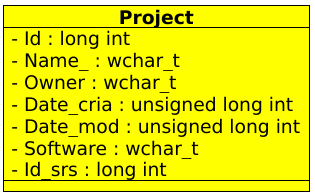
\includegraphics[width=0.5\hsize]{figuras/31.png}
  %\legend{Texto da legenda quando necessário.}
  \source{A autora, 2019.}
\end{figure}

\begin{figure}[!ht]{5cm}
  \caption{Classe Srs} \label{srs}
  \centering
  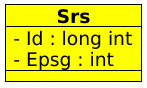
\includegraphics[width=0.5\hsize]{figuras/33.png}
  %\legend{Texto da legenda quando necessário.}
  \source{A autora, 2019.}
\end{figure}

\begin{figure}[!ht]{6cm}
  \caption{Classe Cg\_central\_area} \label{cg}
  \centering
  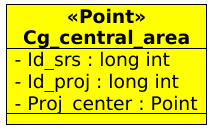
\includegraphics[width=0.6\hsize]{figuras/32.png}
  %\legend{Texto da legenda quando necessário.}
  \source{A autora, 2019.}
\end{figure}

\begin{figure}[!ht]{6cm}
  \caption{Classe Terrain} \label{terrain}
  \centering
  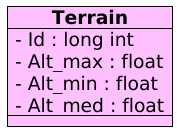
\includegraphics[width=0.6\hsize]{figuras/37.png}
  %\legend{Texto da legenda quando necessário.}
  \source{A autora, 2019.}
\end{figure}

\begin{figure}[!ht]{10cm}
  \caption{Classe Flight} \label{flight}
  \centering
  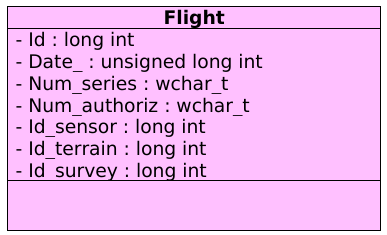
\includegraphics[width=0.6\hsize]{figuras/34.png}
  %\legend{Texto da legenda quando necessário.}
  \source{A autora, 2019.}
\end{figure}

\begin{figure}[!ht]{10cm}
  \caption{Classe Param\_flight} \label{parm_flight}
  \centering
  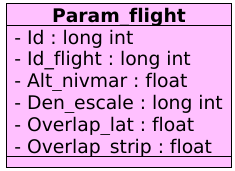
\includegraphics[width=0.5\hsize]{figuras/35.png}
  %\legend{Texto da legenda quando necessário.}
  \source{A autora, 2019.}
\end{figure}

\begin{figure}[!ht]{6cm}
  \caption{Classe Bouding\_box} \label{bbox}
  \centering
  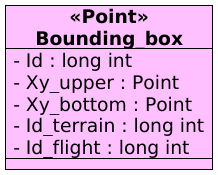
\includegraphics[width=0.7\hsize]{figuras/36.png}
  %\legend{Texto da legenda quando necessário.}
  \source{A autora, 2019.}
\end{figure}

\begin{figure}[!ht]{6cm}
  \caption{Classe Sensor} \label{sensor}
  \centering
  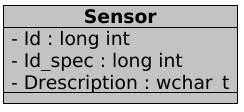
\includegraphics[width=0.8\hsize]{figuras/41.png}
  %\legend{Texto da legenda quando necessário.}
  \source{A autora, 2019.}
\end{figure}

\begin{figure}[!ht]{10cm}
  \caption{Classe Specification} \label{spec}
  \centering
  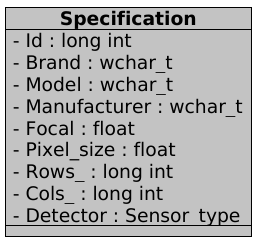
\includegraphics[width=0.5\hsize]{figuras/42.png}
  %\legend{Texto da legenda quando necessário.}
  \source{A autora, 2019.}
\end{figure}

\begin{figure}[!ht]{10cm}
  \caption{Data type Sensor\_type } \label{typesensor}
  \centering
  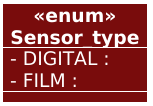
\includegraphics[width=0.4\hsize]{figuras/45.png}
  %\legend{Texto da legenda quando necessário.}
  \source{A autora, 2019.}
\end{figure}

\begin{figure}[!ht]{10cm}
  \caption{Classe Calibration} \label{calib}
  \centering
  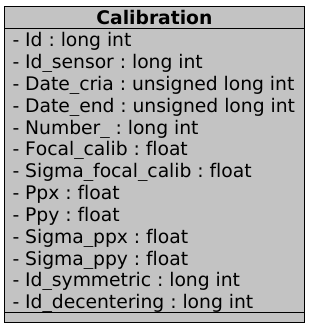
\includegraphics[width=0.6\hsize]{figuras/39.png}
  %\legend{Texto da legenda quando necessário.}
  \source{A autora, 2019.}
\end{figure}

\begin{figure}[!ht]{6cm}
  \caption{Classe Fiducials} \label{fid}
  \centering
  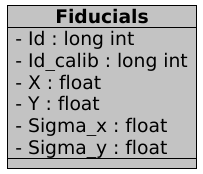
\includegraphics[width=0.75\hsize]{figuras/38.png}
  %\legend{Texto da legenda quando necessário.}
  \source{A autora, 2019.}
\end{figure}

\begin{figure}[!ht]{10cm}
  \caption{Classe Symmetric\_distortion} \label{sym}
  \centering
  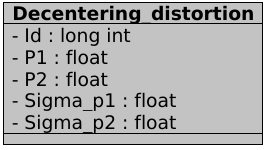
\includegraphics[width=0.5\hsize]{figuras/43.png}
  %\legend{Texto da legenda quando necessário.}
  \source{A autora, 2019.}
\end{figure}

\begin{figure}[!ht]{6cm}
  \caption{Classe Decentering\_distortion} \label{dis}
  \centering
  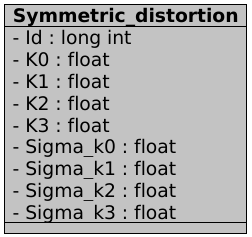
\includegraphics[width=0.75\hsize]{figuras/40.png}
  %\legend{Texto da legenda quando necessário.}
  \source{A autora, 2019.}
\end{figure}

\begin{figure}[!ht]{6cm}
  \caption{Classe Point} \label{point}
  \centering
  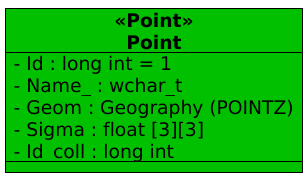
\includegraphics[width=1\hsize]{figuras/30.png}
  %\legend{Texto da legenda quando necessário.}
  \source{A autora, 2019.}
\end{figure}

\begin{figure}[!ht]{10cm}
  \caption{Classe Collection\_Point} \label{collpoint}
  \centering
  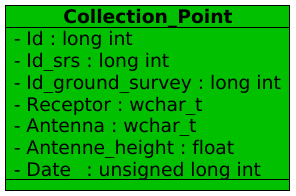
\includegraphics[width=0.6\hsize]{figuras/29.png}
  %\legend{Texto da legenda quando necessário.}
  \source{A autora, 2019.}
\end{figure}

\begin{figure}[!ht]{6cm}
  \caption{Classe Point\_project} \label{pointpro}
  \centering
  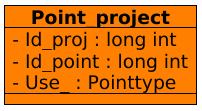
\includegraphics[width=0.8\hsize]{figuras/22.png}
  %\legend{Texto da legenda quando necessário.}
  \source{A autora, 2019.}
\end{figure}

\begin{figure}[!ht]{6cm}
  \caption{Data type Pointtype} \label{pointype}
  \centering
  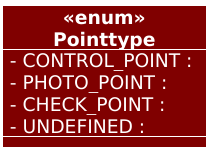
\includegraphics[width=0.8\hsize]{figuras/24.png}
  %\legend{Texto da legenda quando necessário.}
  \source{A autora, 2019.}
\end{figure}

\begin{figure}[!ht]{6cm}
  \caption{Classe Ground\_survey} \label{gp}
  \centering
  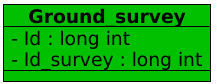
\includegraphics[width=0.8\hsize]{figuras/27.png}
  %\legend{Texto da legenda quando necessário.}
  \source{A autora, 2019}
\end{figure}

\begin{figure}[!ht]{6cm}
  \caption{Classe Measure} \label{meas}
  \centering
  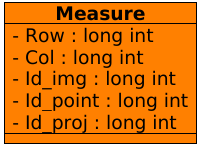
\includegraphics[width=0.6\hsize]{figuras/21.png}
  %\legend{Texto da legenda quando necessário.}
  \source{A autora, 2019}
\end{figure}

\begin{figure}[!ht]{10cm}
  \caption{Classe Image} \label{img}
  \centering
  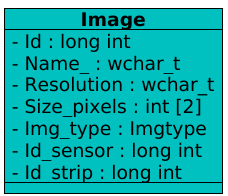
\includegraphics[width=0.5\hsize]{figuras/6.png}
  %\legend{Texto da legenda quando necessário.}
  \source{A autora, 2019}
\end{figure}

\begin{figure}[!ht]{6cm}
  \caption{Data type Imgtype} \label{imgt}
  \centering
  
\includegraphics[width=0.8\hsize]{figuras/25.png}
  %\legend{Texto da legenda quando necessário.}
  \source{A autora, 2019}
\end{figure}

\begin{figure}[!ht]{6cm}
  \caption{Classe File\_img} \label{file}
  \centering
  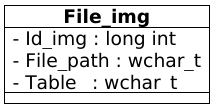
\includegraphics[width=0.75\hsize]{figuras/19.png}
  %\legend{Texto da legenda quando necessário.}
  \source{A autora, 2019}
\end{figure}

\begin{figure}[!ht]{6cm}
  \caption{Classe Tn} \label{tn}
  \centering
  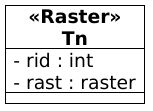
\includegraphics[width=0.55\hsize]{figuras/18.png}
  %\legend{Texto da legenda quando necessário.}
  \source{A autora, 2019}
\end{figure}

\begin{figure}[!ht]{6cm}
  \caption{Classe Photo} \label{photo}
  \centering
  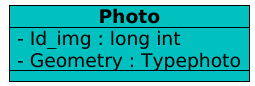
\includegraphics[width=0.8\hsize]{figuras/3.png}
  %\legend{Texto da legenda quando necessário.}
  \source{A autora, 2019}
\end{figure}

\begin{figure}[!ht]{6cm}
  \caption{Data type Typephoto} \label{tp}
  \centering
  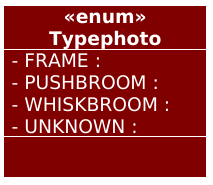
\includegraphics[width=0.8\hsize]{figuras/26.png}
  %\legend{Texto da legenda quando necessário.}
  \source{A autora, 2019}
\end{figure}

\begin{figure}[!ht]{6cm}
  \caption{Classe Frame} \label{fram}
  \centering
  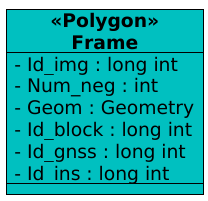
\includegraphics[width=0.75\hsize]{figuras/2.png}
  %\legend{Texto da legenda quando necessário.}
  \source{A autora, 2019}
\end{figure}

\begin{figure}[!ht]{6cm}
  \caption{Classe Strip} \label{strip}
  \centering
  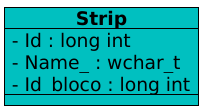
\includegraphics[width=0.7\hsize]{figuras/16.png}
  %\legend{Texto da legenda quando necessário.}
  \source{A autora, 2019}
\end{figure}

\begin{figure}[!ht]{6cm}
  \caption{Classe Block} \label{blo}
  \centering
  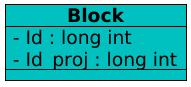
\includegraphics[width=0.65\hsize]{figuras/17.png}
  %\legend{Texto da legenda quando necessário.}
  \source{A autora, 2019}
\end{figure}

\begin{figure}[!ht]{6cm}
  \caption{Classe Img\_block} \label{imgblo}
  \centering
  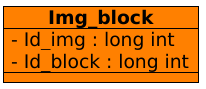
\includegraphics[width=0.7\hsize]{figuras/20.png}
  %\legend{Texto da legenda quando necessário.}
  \source{A autora, 2019}
\end{figure}

\begin{figure}[!ht]{6cm}
  \caption{Classe Pair} \label{pair}
  \centering
  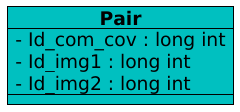
\includegraphics[width=0.75\hsize]{figuras/8.png}
  %\legend{Texto da legenda quando necessário.}
  \source{A autora, 2019}
\end{figure}

\begin{figure}[!ht]{6cm}
  \caption{Classe Coverage} \label{comm}
  \centering
  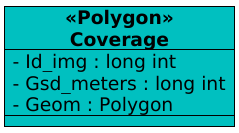
\includegraphics[width=0.75\hsize]{figuras/5.png}
  %\legend{Texto da legenda quando necessário.}
  \source{A autora, 2019}
\end{figure}

\begin{figure}[!ht]{6cm}
  \caption{Classe Common\_coverage} \label{comcov}
  \centering
  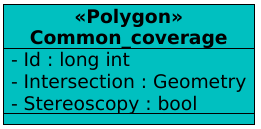
\includegraphics[width=0.85\hsize]{figuras/9.png}
  %\legend{Texto da legenda quando necessário.}
  \source{A autora, 2019}
\end{figure}

\begin{figure}[!ht]{6cm}
  \caption{Classe Ntuplet} \label{ntu}
  \centering
  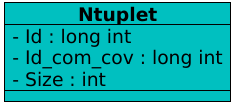
\includegraphics[width=0.7\hsize]{figuras/12.png}
  %\legend{Texto da legenda quando necessário.}
  \source{A autora, 2019}
\end{figure}

\begin{figure}[!ht]{6cm}
  \caption{Classe Img\_ntuplet} \label{imgtu}
  \centering
  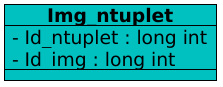
\includegraphics[width=0.7\hsize]{figuras/14.png}
  %\legend{Texto da legenda quando necessário.}
  \source{A autora, 2019}
\end{figure}

\begin{figure}[!ht]{6cm}
  \caption{Classe Mod\_param} \label{modpar}
  \centering
  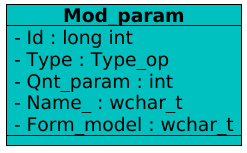
\includegraphics[width=0.7\hsize]{figuras/11.png}
  %\legend{Texto da legenda quando necessário.}
  \source{A autora, 2019}
\end{figure}

\begin{figure}[!ht]{6cm}
  \caption{Data type Type\_op} \label{top}
  \centering
  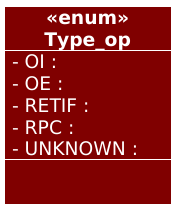
\includegraphics[width=0.6\hsize]{figuras/23.png}
  %\legend{Texto da legenda quando necessário.}
  \source{A autora, 2019}
\end{figure}

\begin{figure}[!ht]{6cm}
  \caption{Classe Parameter} \label{par}
  \centering
  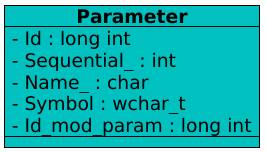
\includegraphics[width=0.7\hsize]{figuras/7.png}
  %\legend{Texto da legenda quando necessário.}
  \source{A autora, 2019}
\end{figure}

\begin{figure}[!ht]{6cm}
  \caption{Classe Coef\_img} \label{coefimg}
  \centering
  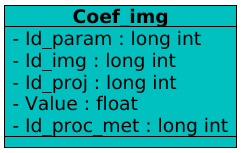
\includegraphics[width=0.8\hsize]{figuras/15.png}
  %\legend{Texto da legenda quando necessário.}
  \source{A autora, 2019}
\end{figure}

\begin{figure}[!ht]{10cm}
  \caption{Classe Processing\_metho} \label{proces}
  \centering
  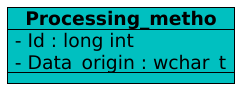
\includegraphics[width=0.5\hsize]{figuras/44.png}
  %\legend{Texto da legenda quando necessário.}
  \source{A autora, 2019}
\end{figure}

\begin{figure}[!ht]{6cm}
  \caption{Classe Frame\_gnss} \label{gnss}
  \centering
  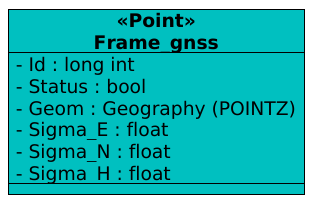
\includegraphics[width=1\hsize]{figuras/1.png}
  %\legend{Texto da legenda quando necessário.}
  \source{A autora, 2019}
\end{figure}

\begin{figure}[!ht]{6cm}
  \caption{Classe Frame\_ins} \label{ins}
  \centering
  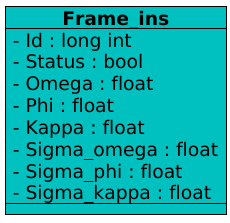
\includegraphics[width=0.65\hsize]{figuras/4.png}
  %\legend{Texto da legenda quando necessário.}
  \source{A autora, 2019}
\end{figure}


\section{Modelos completos}\label{ap-1}
\begin{landscape}
\begin{figure}[ht]{21cm}
  \caption{Modelo Orientado à Objeto.} \label{modelo_00}
  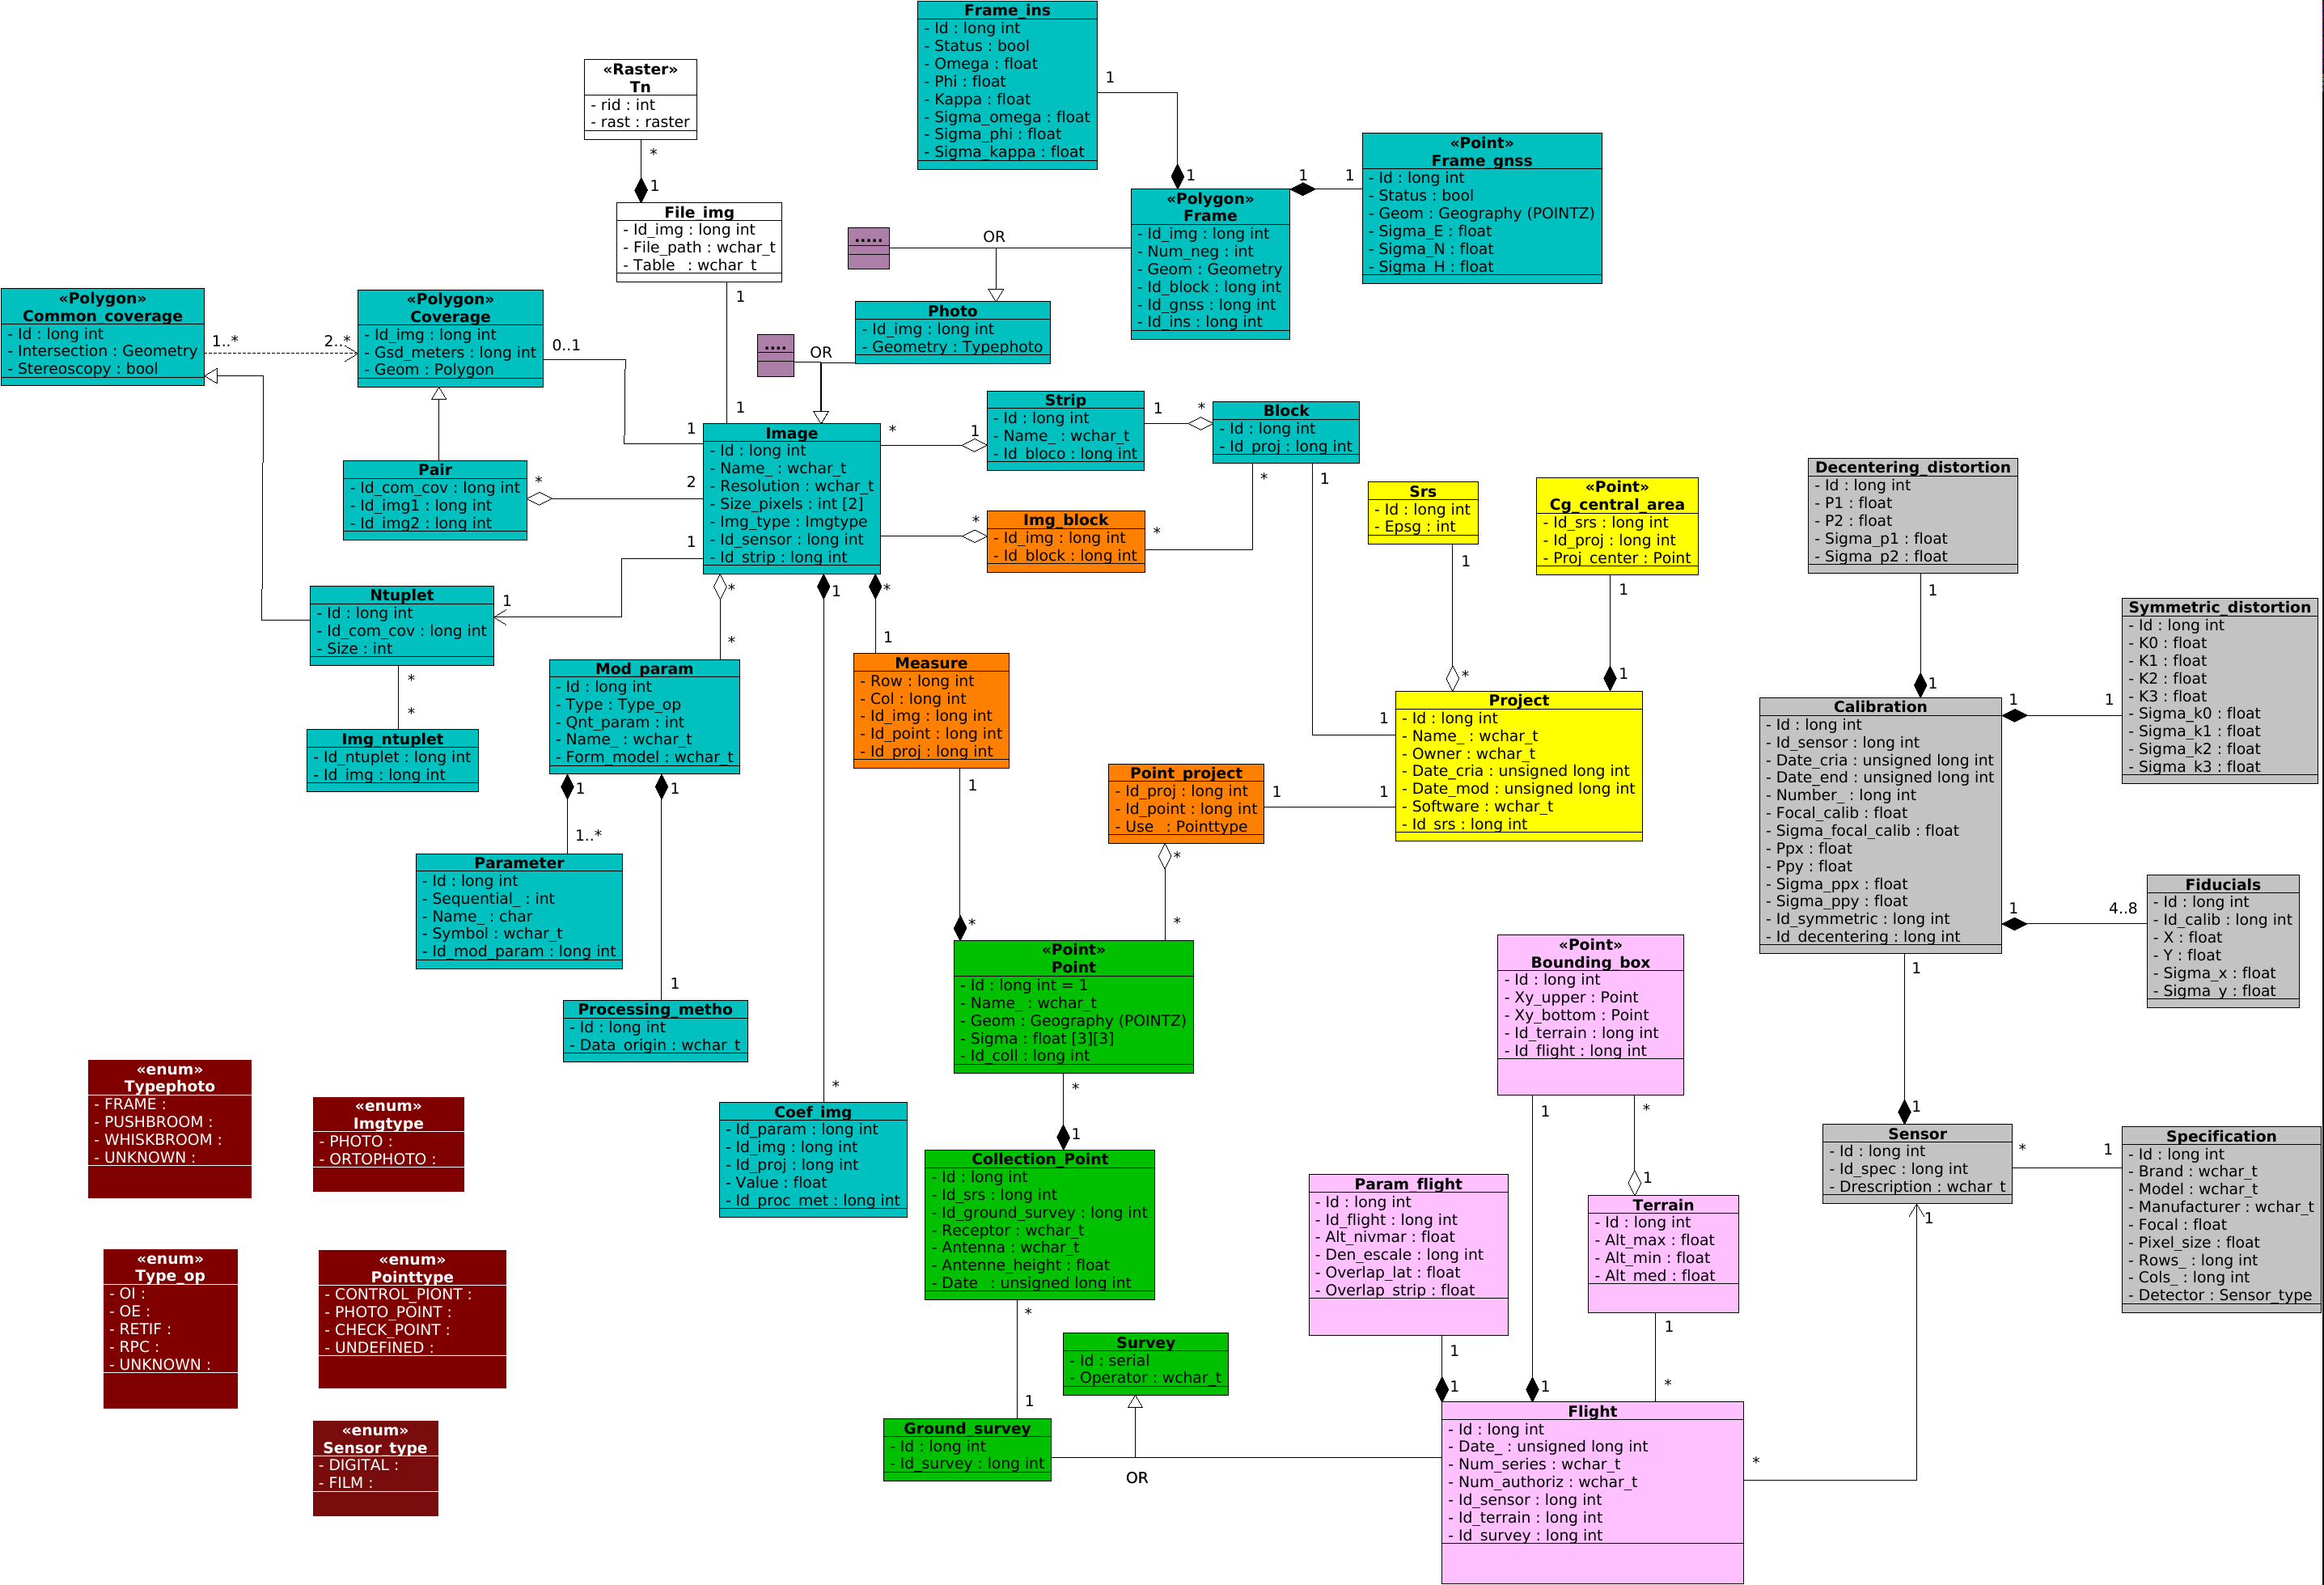
\includegraphics[width=\hsize]{figuras/modelo_oo.png}
  \legend{Imagem gerada com o software Umbrello.}
  \source{A autora, 2019}
\end{figure}
\end{landscape}

\begin{landscape}
\begin{figure}[ht]{25cm}
  \caption{Modelo Relacional.} \label{modelo_r}
  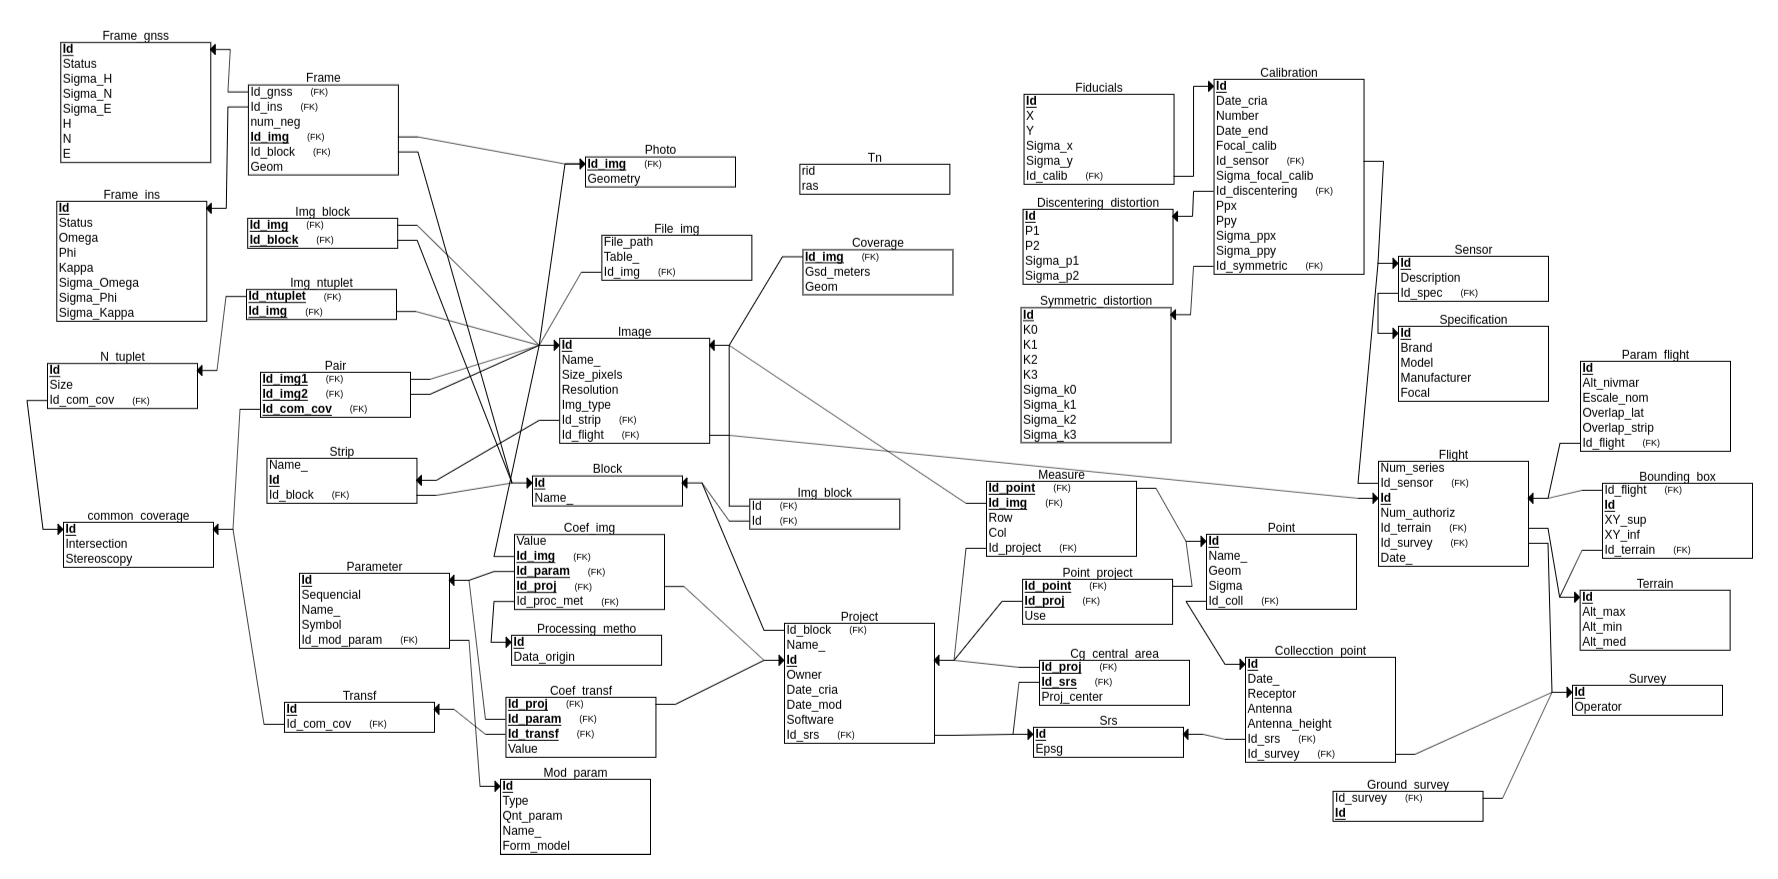
\includegraphics[width=\hsize]{figuras/modelo_er.png}
  \legend{Imagem gerada com a plataforma online ERDPlus.}
  \source{A autora, 2019}
\end{figure}
\end{landscape}





%=====================================================================
\postextualchapter{Códigos}\label{ap1}
%=====================================================================
\section{Código para o Banco de Dados}\label{cdg}

Código para a criação do Projeto Piloto do Banco de Dados.
\lstinputlisting[]{codigos/cdgbanco.sql}

\section{Cargas}\label{crg}
Código de cargas realizadas no banco
\subsection{Primeira Carga} \label{carga1}
\lstinputlisting[]{codigos/carga1.sql}
\subsection{Segunda Carga}\label{carga2}
\lstinputlisting[]{codigos/carga2.sql}
\subsection{Terceira Carga}\label{carga3}
\lstinputlisting[]{codigos/carga_img.sh}

\section{Consultas}\label{con}
Código das funções e visões usadas para testar o Banco de Dados
\subsection{Visões}\label{visoes}
\lstinputlisting[]{codigos/quest_views.sql}
\subsection{Funções}\label{funcoes}
\lstinputlisting[]{codigos/quest_functions.sql}

